
An RPN (Reverse Polish Notation) calculator is a stack-based calculator that uses postfix notation, where the operator follows the operands. It's commonly used in printing calculators and, notably, the HP 12C, the most popular electronic calculator of all time.

After becoming familiar with its operational modality, many people prefer an RPN calculator. (I've been using the HP 12C and 16C since they were first introduced in the early 1980s.) For example, using conventional algebraic notation, to add 1 and 2 you would type 1 + 2. Using RPN, you would type 1 2 +. The operator comes after the operands.

Using an algebraic calculator, you would need to press an = key to indicate that you want a result. With an RPN calculator this is unnecessary because the operator processes immediately, serving a double purpose. On the other hand, an RPN calculator often requires an Enter keypress to push an operand onto the stack.

We can easily implement an RPN calculator using a stack-based data structure.
For example, consider an RPN calculator with a four-position stack:

\hspace*{\fill} \\ %插入空行
\begin{center}
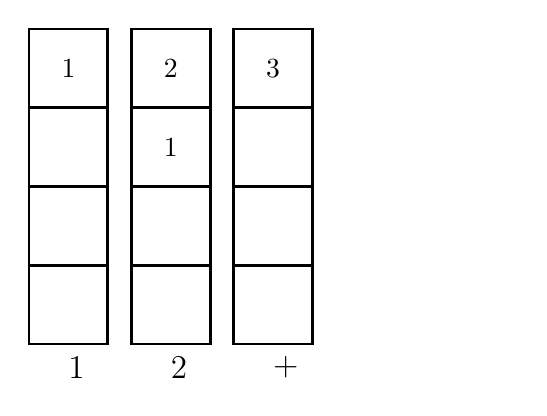
\begin{tikzpicture}
\draw[line width=1pt] (1,-1*0) rectangle (0, -1*0+1) node[pos=.5] {1};
\draw[line width=1pt] (1,-1*1) rectangle (0, -1*1+1);
\draw[line width=1pt] (1,-1*2) rectangle (0, -1*2+1);
\draw[line width=1pt] (1,-1*3) rectangle (0, -1*3+1);

\draw[line width=1pt] (2.3,-1*0) rectangle (1.3, -1*0+1) node[pos=.5] {2};
\draw[line width=1pt] (2.3,-1*1) rectangle (1.3, -1*1+1) node[pos=.5] {1};
\draw[line width=1pt] (2.3,-1*2) rectangle (1.3, -1*2+1);
\draw[line width=1pt] (2.3,-1*3) rectangle (1.3, -1*3+1);

\draw[line width=1pt] (3.6,-1*0) rectangle (2.6, -1*0+1) node[pos=.5] {3};
\draw[line width=1pt] (3.6,-1*1) rectangle (2.6, -1*1+1);
\draw[line width=1pt] (3.6,-1*2) rectangle (2.6, -1*2+1);
\draw[line width=1pt] (3.6,-1*3) rectangle (2.6, -1*3+1);

\node[text width=3cm, font=\large] at (2,-3.3) {1};
\node[text width=3cm, font=\large] at (3.3,-3.3) {2};
\node[text width=3cm, font=\large] at (4.6,-3.3) {+};
\end{tikzpicture}
	
Figure 3.5 – RPN addition operation
\end{center}

Each operand is pushed onto the stack as they are entered. When the operator is entered, the operands are popped off, operated upon, and the result is pushed back onto the stack. The result may then be used in the next operation. For example, consider the case of (3+2)×3:

\hspace*{\fill} \\ %插入空行
\begin{center}
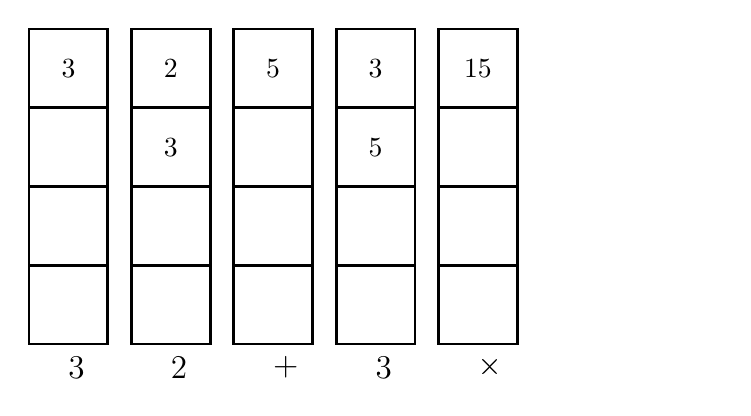
\begin{tikzpicture}
\draw[line width=1pt] (1,-1*0) rectangle (0, -1*0+1) node[pos=.5] {3};
\draw[line width=1pt] (1,-1*1) rectangle (0, -1*1+1);
\draw[line width=1pt] (1,-1*2) rectangle (0, -1*2+1);
\draw[line width=1pt] (1,-1*3) rectangle (0, -1*3+1);

\draw[line width=1pt] (2.3,-1*0) rectangle (1.3, -1*0+1) node[pos=.5] {2};
\draw[line width=1pt] (2.3,-1*1) rectangle (1.3, -1*1+1) node[pos=.5] {3};
\draw[line width=1pt] (2.3,-1*2) rectangle (1.3, -1*2+1);
\draw[line width=1pt] (2.3,-1*3) rectangle (1.3, -1*3+1);

\draw[line width=1pt] (3.6,-1*0) rectangle (2.6, -1*0+1) node[pos=.5] {5};
\draw[line width=1pt] (3.6,-1*1) rectangle (2.6, -1*1+1);
\draw[line width=1pt] (3.6,-1*2) rectangle (2.6, -1*2+1);
\draw[line width=1pt] (3.6,-1*3) rectangle (2.6, -1*3+1);

\draw[line width=1pt] (4.9,-1*0) rectangle (3.9, -1*0+1) node[pos=.5] {3};
\draw[line width=1pt] (4.9,-1*1) rectangle (3.9, -1*1+1) node[pos=.5] {5};
\draw[line width=1pt] (4.9,-1*2) rectangle (3.9, -1*2+1);
\draw[line width=1pt] (4.9,-1*3) rectangle (3.9, -1*3+1);

\draw[line width=1pt] (6.2,-1*0) rectangle (5.2, -1*0+1) node[pos=.5] {15};
\draw[line width=1pt] (6.2,-1*1) rectangle (5.2, -1*1+1);
\draw[line width=1pt] (6.2,-1*2) rectangle (5.2, -1*2+1);
\draw[line width=1pt] (6.2,-1*3) rectangle (5.2, -1*3+1);

\node[text width=3cm, font=\large] at (2,-3.3) {3};
\node[text width=3cm, font=\large] at (3.3,-3.3) {2};
\node[text width=3cm, font=\large] at (4.6,-3.3) {+};
\node[text width=3cm, font=\large] at (5.9,-3.3) {3};
\node[text width=3cm, font=\large] at (7.2,-3.3) {×};
\end{tikzpicture}

Figure 3.6 – RPN stack operations
\end{center}

One advantage of RPN is that you can leave operands on the stack for future calculations, reducing the need for separate memory registers. Consider the case of (9×6)+(2×3):

\hspace*{\fill} \\ %插入空行
\begin{center}
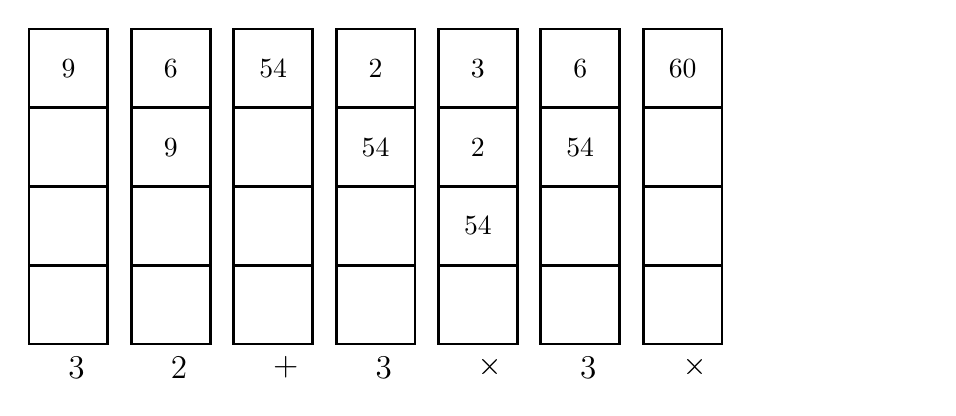
\begin{tikzpicture}
\draw[line width=1pt] (1,-1*0) rectangle (0, -1*0+1) node[pos=.5] {9};
\draw[line width=1pt] (1,-1*1) rectangle (0, -1*1+1);
\draw[line width=1pt] (1,-1*2) rectangle (0, -1*2+1);
\draw[line width=1pt] (1,-1*3) rectangle (0, -1*3+1);

\draw[line width=1pt] (2.3,-1*0) rectangle (1.3, -1*0+1) node[pos=.5] {6};
\draw[line width=1pt] (2.3,-1*1) rectangle (1.3, -1*1+1) node[pos=.5] {9};
\draw[line width=1pt] (2.3,-1*2) rectangle (1.3, -1*2+1);
\draw[line width=1pt] (2.3,-1*3) rectangle (1.3, -1*3+1);

\draw[line width=1pt] (3.6,-1*0) rectangle (2.6, -1*0+1) node[pos=.5] {54};
\draw[line width=1pt] (3.6,-1*1) rectangle (2.6, -1*1+1);
\draw[line width=1pt] (3.6,-1*2) rectangle (2.6, -1*2+1);
\draw[line width=1pt] (3.6,-1*3) rectangle (2.6, -1*3+1);

\draw[line width=1pt] (4.9,-1*0) rectangle (3.9, -1*0+1) node[pos=.5] {2};
\draw[line width=1pt] (4.9,-1*1) rectangle (3.9, -1*1+1) node[pos=.5] {54};
\draw[line width=1pt] (4.9,-1*2) rectangle (3.9, -1*2+1);
\draw[line width=1pt] (4.9,-1*3) rectangle (3.9, -1*3+1);

\draw[line width=1pt] (6.2,-1*0) rectangle (5.2, -1*0+1) node[pos=.5] {3};
\draw[line width=1pt] (6.2,-1*1) rectangle (5.2, -1*1+1) node[pos=.5] {2};
\draw[line width=1pt] (6.2,-1*2) rectangle (5.2, -1*2+1) node[pos=.5] {54};
\draw[line width=1pt] (6.2,-1*3) rectangle (5.2, -1*3+1);

\draw[line width=1pt] (7.5,-1*0) rectangle (6.5, -1*0+1) node[pos=.5] {6};
\draw[line width=1pt] (7.5,-1*1) rectangle (6.5, -1*1+1) node[pos=.5] {54};
\draw[line width=1pt] (7.5,-1*2) rectangle (6.5, -1*2+1);
\draw[line width=1pt] (7.5,-1*3) rectangle (6.5, -1*3+1);

\draw[line width=1pt] (8.8,-1*0) rectangle (7.8, -1*0+1) node[pos=.5] {60};
\draw[line width=1pt] (8.8,-1*1) rectangle (7.8, -1*1+1);
\draw[line width=1pt] (8.8,-1*2) rectangle (7.8, -1*2+1);
\draw[line width=1pt] (8.8,-1*3) rectangle (7.8, -1*3+1);

\node[text width=3cm, font=\large] at (2,-3.3) {3};
\node[text width=3cm, font=\large] at (3.3,-3.3) {2};
\node[text width=3cm, font=\large] at (4.6,-3.3) {+};
\node[text width=3cm, font=\large] at (5.9,-3.3) {3};
\node[text width=3cm, font=\large] at (7.2,-3.3) {×};
\node[text width=3cm, font=\large] at (8.5,-3.3) {3};
\node[text width=3cm, font=\large] at (9.8,-3.3) {×};
\end{tikzpicture}

Figure 3.7 – RPN multiple stack operations
\end{center}

Notice that we first perform the operations within the parentheses, then the final operation on the intermediate results. This may seem more complex at first, but it makes a lot of sense once you get used to it.

Now, let's build a simple RPN calculator using the STL deque container.

\subsubsection{How to do it…}

For this implementation, we'll use a deque container for our stack. Why not use a stack container? The stack class is a container-adapter, which uses another container (usually a deque) for its storage. For our purposes, stack doesn't provide any tangible advantage over deque. And deque allows us to iterate over and display the RPN stack, like a paper tape calculator.

\begin{itemize}
\item 
We'll encapsulate our RPN calculator in a class. There are a few advantages to using a class here. Encapsulation provides safety, reusability, extensibility, and a clean interface. We'll call our class RPN:

\begin{lstlisting}[style=styleCXX]
class RPN {
	deque<double> deq_{};
	constexpr static double zero_{0.0};
	constexpr static double inf_
		{ std::numeric_limits<double>::infinity() };
... // public and private members go here
};
\end{lstlisting}

The deque data store, named deq\_, is in the private area of the class to protect it.
This is where we store the RPN stack.

The zero\_ constant is used throughout the class, both as a return value and as a comparison operand. The inf\_ constant is used for a divide-by-zero error. These constants are declared constexpr static so they don't take up space in every instance.

I like to name private data members with a trailing underscore to remind me that they're private.

\item 
We don't need an explicit constructor or destructor because the deque class manages its own resources. So, our public interface consists of just three functions:

\begin{lstlisting}[style=styleCXX]
public:
	// process an operand/operator
	double op(const string & s) {
		if(is_numeric(s)) {
			double v{stod(s, nullptr)};
			deq_.push_front(v);
			return v;
		}
		else return optor(s);
	}
	// empty the stack
	void clear() {
		deq_.clear();
	}
	// print the stack
	string get_stack_string() const {
		string s{};
		for(auto v : deq_) {
			s += format("{} ", v);
		}
		return s;
	}
\end{lstlisting}

The double op() function is the main entry point for the RPN class. It takes a string, with either a number or an operator. If it's a number, it's converted into a double and pushed onto the stack. If it's an operator, we call optor() to perform the operation. This is the main logic of the class.

The void clear() function simply calls clear() on the deque to empty the stack.

And finally, the string get\_stack\_string() function returns the contents of the stack in a string.

\item 
In the private section, we have the supporting utilities that make the interface work. The pop\_get2() function pops two operands from the stack and returns them as a pair. We use this as operands for the operators:

\begin{lstlisting}[style=styleCXX]
pair<double, double> pop_get2() {
	if(deq_.size() < 2) return {zero_, zero_};
	double v1{deq_.front()};
	deq_.pop_front();
	double v2{deq_.front()};
	deq_.pop_front();
	return {v2, v1};
}
\end{lstlisting}

\item 
The is\_numeric() function checks to see if the string is entirely numeric. We also allow the decimal . character

\begin{lstlisting}[style=styleCXX]
bool is_numeric(const string& s) {
	for(const char c : s) {
		if(c != '.' && !std::isdigit(c)) return
		false;
	}
	return true;
}
\end{lstlisting}

\item 
The optor() function performs the operators. We use a map container to map an operator to a corresponding lambda function.

\begin{lstlisting}[style=styleCXX]
double optor(const string& op) {
	map<string, double (*)(double, double)> opmap {
		{"+", [](double l, double r){ return l + r; }},
		{"-", [](double l, double r){ return l - r; }},
		{"*", [](double l, double r){ return l * r; }},
		{"/", [](double l, double r){ return l / r; }},
		{"^", [](double l, double r)
			{ return pow(l, r); }},
		{"%", [](double l, double r)
			{ return fmod(l, r); }}
	};
	if(opmap.find(op) == m.end()) return zero_;
	auto [l, r] = pop_get2();
	// don’t divide by zero
	if(op == "/" && r == zero_) deq_.push_front(inf_);
	else deq_.push_front(opmap.at(op)(l, r));
	return deq_.front();
}
\end{lstlisting}

The map container with lambda functions makes a quick and easy jump table.

We use the find() function in map to test if we have a valid operator.

After a test for divide-by-zero, the map is dereferenced, and the operator is called.

The result of the operation is pushed onto the stack and returned.

\item 
Those are all the function members of the RPN class. Now we can use it in our main() function:

\begin{lstlisting}[style=styleCXX]
int main() {
	RPN rpn;
	
	for(string o{}; cin >> o; ) {
		rpn.op(o);
		auto stack_str{rpn.get_stack_string()};
		cout << format("{}: {}\n", o, stack_str);
	}
}
\end{lstlisting}

We'll test this is by piping a string into the program from the command line. We use a for loop to fetch each word from the cin stream and pass it to rpn.op(). I like the for loop here, as it's easy to contain the scope of the o variable. We then print the stack using the get\_stack\_string() function after each command line item.


\item 
We can run the program by piping in an expression like this:

\begin{tcblisting}{commandshell={}}
$ echo "9 6 * 2 3 * +" | ./rpn
9: 9
6: 6 9
*: 54
2: 2 54
3: 3 2 54
*: 6 54
+: 60
\end{tcblisting}
\end{itemize}

This looks like a lot of coding but it's actually quite simple. With the comments, the RPN class is less than 70 lines of code. The full rpn.cpp source code is in the GitHub repository.

\subsubsection{How it works…}

The RPN class operates by first determining the nature of each chunk of input. If it's a number, we push it onto the stack. If it's an operator, we pop two operands off the top of the stack, apply the operation, and push the result back on the stack. If we don't recognize the input, we just ignore it.

The deque class is a double-ended queue. To use it as a stack, we pick an end and both push and pop from that same end. I chose the front end of the deque, but it would work just as well from the back. We just need to do everything from the same end.

If we determine that an input is numeric, we convert it to a double and push it onto the front of the deque using push\_front().

\begin{lstlisting}[style=styleCXX]
if(is_numeric(s)) {
	double v{stod(s, nullptr)};
	deq_.push_front(v);
	return v;
}
\end{lstlisting}

When we need to use values from the stack, we pop them off the front of the deque. We use front() to get the value, and then pop\_front() to pop it off the stack.

\begin{lstlisting}[style=styleCXX]
pair<double, double> pop_get2() {
	if(deq_.size() < 2) return {zero_, zero_};
	double v1{deq_.front()};
	deq_.pop_front();
	double v2{deq_.front()};
	deq_.pop_front();
	return {v2, v1};
}
\end{lstlisting}

Using a map for our operators makes it easy to both check if an operator is valid, and to execute the operation.

\begin{lstlisting}[style=styleCXX]
map<string, double (*)(double, double)> opmap {
	{"+", [](double l, double r){ return l + r; }},
	{"-", [](double l, double r){ return l - r; }},
	{"*", [](double l, double r){ return l * r; }},
	{"/", [](double l, double r){ return l / r; }},
	{"^", [](double l, double r){ return pow(l, r); }},
	{"%", [](double l, double r){ return fmod(l, r); }}
};
\end{lstlisting}

We can test for the validity of an operator by using the find() function:

\begin{lstlisting}[style=styleCXX]
if(opmap.find(op) == opmap.end()) return zero_;
\end{lstlisting}

And we can call the operator by dereferencing the map with the at() function:

\begin{lstlisting}[style=styleCXX]
opmap.at(op)(l, r)
\end{lstlisting}

We both call the operator lambda and push the result onto the deque in one statement:

\begin{lstlisting}[style=styleCXX]
deq_.push_front(opmap.at(op)(l, r));
\end{lstlisting}

\subsubsection{There's more…}

In this recipe, we use the cin stream to feed operations to the RPN calculator. It would be just as easy to do this with an STL container.

\begin{lstlisting}[style=styleCXX]
int main() {
	RPN rpn;
	vector<string> opv{ "9", "6", "*", "2", "3", "*", "+"
	};
	for(auto o : opv) {
		rpn.op(o);
		auto stack_str{rpn.get_stack_string()};
		cout << format("{}: {}\n", o, stack_str);
	}
}
\end{lstlisting}

Output:

\begin{tcblisting}{commandshell={}}
9: 9
6: 6 9
*: 54
2: 2 54
3: 3 2 54
*: 6 54
+: 60
\end{tcblisting}

By putting the RPN calculator in a class with a clean interface, we've created a flexible tool that can be used in many different contexts.







